% CLAUDE REPORT::WCD-REGIMES-0001::2026-11-14T14:00-08:00
% Claude routine "worst-case minimum derivation cost". User follow-up: pairwise limits of k, n, m, T, S, and FLMV slices.
% Role-neutral and additive. It does NOT edit root main.tex or any TMR/LSPV region.
\documentclass[11pt]{article}
\usepackage{amsmath,amssymb,amsthm,graphicx,booktabs,longtable}
\usepackage[margin=0.9in]{geometry}
\newtheorem{lemma}{Lemma}
\title{WCD-REGIMES-0001: pairwise limits of $k,n,m,T,S$ for $k$-SAT, and slices of the FLMV region}
\author{Claude scheduled routine (worst-case derivation complexity log)}
\date{2026-11-14 14:00 America/Los\_Angeles}
\begin{document}
\maketitle

\paragraph{Status line.}
\begin{itemize}
\item Lemmas~\ref{lem:union}--\ref{lem:dense}: \textbf{PROVED/EXACT} (elementary).
\item Table entries are labelled individually. Every \textbf{KNOWN THEOREM} entry is cited from memory and was not re-read this run.
\item The figure's frontier is the checkpoint scheme of WCD-TWOWORLDS-0001 (\textbf{PROVED/EXACT}); the Williams endpoint and the corpus box are cited, not derived.
\item No new lower bound is claimed. P versus NP remains \textbf{OPEN}.
\end{itemize}

\section{Conventions}
$k$ is clause width, $n$ the number of variables, $m$ the number of distinct clauses, and $L\approx mk\log n$ the input length in bits. $T$ and $S$ are the time and space of a deterministic machine, measured against $L$. The parameters $k,n,m$ are only sent to $\infty$. ``$T\to0$'' means $T=o(L)$, and ``$S\to0$'' means $S=O(1)$ bits; literal zero is meaningless.

\section{Three elementary lemmas}
\begin{lemma}[union bound]\label{lem:union}
If every clause has $k$ distinct variables and $m<2^{k}$, the formula is satisfiable.
\end{lemma}
\begin{proof}
Each clause is falsified by $2^{n-k}$ assignments, and $m\,2^{n-k}<2^{n}$.
\end{proof}

\begin{lemma}[sublinear time is impossible]\label{lem:skip}
No machine decides $k$-SAT with $T=o(m)$ clause reads on all inputs, for $k\ge2$.
\end{lemma}
\begin{proof}
Take a minimally unsatisfiable formula with $m$ clauses. A machine reading fewer than $m$ clauses misses some clause $C$. Replacing $C$ by a copy of another clause leaves every read clause unchanged and yields a satisfiable formula. One answer is wrong.
\end{proof}

\begin{lemma}[few variables are easy]\label{lem:dense}
Brute force runs in time $2^{n}\mathrm{poly}(L)$ and space $n+O(\log L)$. Hence if $n\le\alpha\log_2L$, SAT is decided in time $L^{\alpha+O(1)}$ and space $O(\log L)$. In particular, any input family that forces time beyond $L^{c}$ in space $L^{o(1)}$ must have $n\ge(c-O(1))\log_2L$.
\end{lemma}
\begin{proof}
Enumerate assignments with an $n$-bit counter and evaluate each clause by scanning the input with $O(\log L)$-bit pointers.
\end{proof}
The exact $O(1)$ depends on the machine model (multitape versus random access); it is not pinned down here.

\section{The table}
\begin{longtable}{p{2.1cm}p{1.6cm}p{8.6cm}p{2.3cm}}
\toprule
Pair & Direction & Effect on the remaining variables & Status\\\midrule
\endhead
$k,n\to\infty$ & & Unsatisfiable needs $m\ge2^{k}$ (Lemma~\ref{lem:union}). If $k\approx n$ then $m\approx2^{n}$, $L\approx n2^{n}$, and brute force is polynomial in $L$; with $k=n$ the problem is counting distinct full clauses. Hardness survives only with $k=o(n)$ and $m$ between $2^{k}$ and about $2^{k}n$. & PROVED; hard band folklore\\
$k,m\to\infty$ & & If $k>\log_2m$ the answer is always ``satisfiable'': constant time. Hardness needs $k\le\log_2m$ and $n\ge k+\omega(\log m)$. & PROVED\\
$n,m\to\infty$ & $k$ fixed & Standard hard regime. NP-hard for $m$ from about $n$ up to $(2n)^{k}$, the most distinct clauses. Random formulas with $m/n\ge n^{k/2-1}\mathrm{polylog}$ are refutable in polynomial time. & KNOWN\\
$k,T$ & $T\to0$ & Only the trivial band $m<2^{k}$; otherwise impossible (Lemma~\ref{lem:skip}). & PROVED\\
$k,T$ & $T\to\infty$ & $T\ge2^{n}\mathrm{poly}(L)$ always suffices. Under SETH, $T\ge2^{(1-o(1))n}$ as $k\to\infty$. & PROVED; SETH conjecture\\
$k,S$ & $S\to0$ & Only the trivial band; otherwise impossible, because constant space recognises only regular languages and SAT is not regular. & KNOWN\\
$k,S$ & $S\to\infty$ & $n+O(\log L)$ bits suffice. & PROVED\\
$n,T$ & $T\to0$ & Impossible (Lemma~\ref{lem:skip}). & PROVED\\
$n,T$ & $T\to\infty$ & $2^{n}\mathrm{poly}(L)$ suffices. Polynomial $T$ is the P versus NP question. & OPEN\\
$n,S$ & $S\to0$ & Constant space impossible. $S=O(\log L)$ would put NP in L. & OPEN\\
$n,S$ & $S\to\infty$ & No time saving from space is known. With $S\ge L$, nothing beyond $T\ge L$ is proved. & OPEN\\
$m,T$ & $T\to0$ & Impossible (Lemma~\ref{lem:skip}). & PROVED\\
$m,T$ & $T\to\infty$ & Fine. With $k$ fixed, $m\to\infty$ forces $n\ge m^{1/k}/2$. & PROVED\\
$m,S$ & $S\to0$ & Impossible in general. If $m$ grows fast enough that $n\le\alpha\log L$, brute force runs in $O(\log L)$ space and polynomial time (Lemma~\ref{lem:dense}). & PROVED\\
$m,S$ & $S\to\infty$ & As for $n,S$. & OPEN\\
$T,S$ & $0,0$ & Impossible. & PROVED\\
$T,S$ & $0,\infty$ & Impossible: sublinear time cannot read the input, whatever the space. & PROVED\\
$T,S$ & $\infty,0$ & Constant space impossible. Logarithmic space open. & KNOWN / OPEN\\
$T,S$ & $\infty,\infty$ & Always decidable. & PROVED\\\midrule
\multicolumn{4}{l}{\emph{The only nontrivial corners}}\\
$T\le L^{1.80}$ & $S=L^{o(1)}$ & Excluded: FLMV, improved by Williams to $2\cos(\pi/7)\approx1.80$. Buss--Williams: alternation trading cannot reach 2 (ledger L13). & KNOWN\\
$T\le L^{1+o(1)}$ & $S=L^{1-\varepsilon}$ & Excluded (Fortnow--van Melkebeek). & KNOWN\\
$T\le L^{c}$ & $S\ge L$ & Not excluded for any $c>1$: no superlinear time bound known. & OPEN\\
\bottomrule
\end{longtable}

\paragraph{Reading.}
\begin{itemize}
\item Every way of sending $k$ or $m$ to infinity on its own reaches a trivial regime: always satisfiable ($k>\log_2m$), or few enough variables for brute force ($n\le\alpha\log L$).
\item Hardness lives on a ridge: $k$ fixed or slowly growing, $m\approx2^{k}n$, $n\to\infty$.
\item On the machine side, every proved superlinear bound needs space below $L$. This is the same boundary met by the checkpoint scheme (WCD-TWOWORLDS-0001), the charged-depth region (WCD-FLMV-0001) and the knowledge-width bound (WCD-REACH-0001).
\end{itemize}

\section{Slices of the FLMV region}
\begin{center}
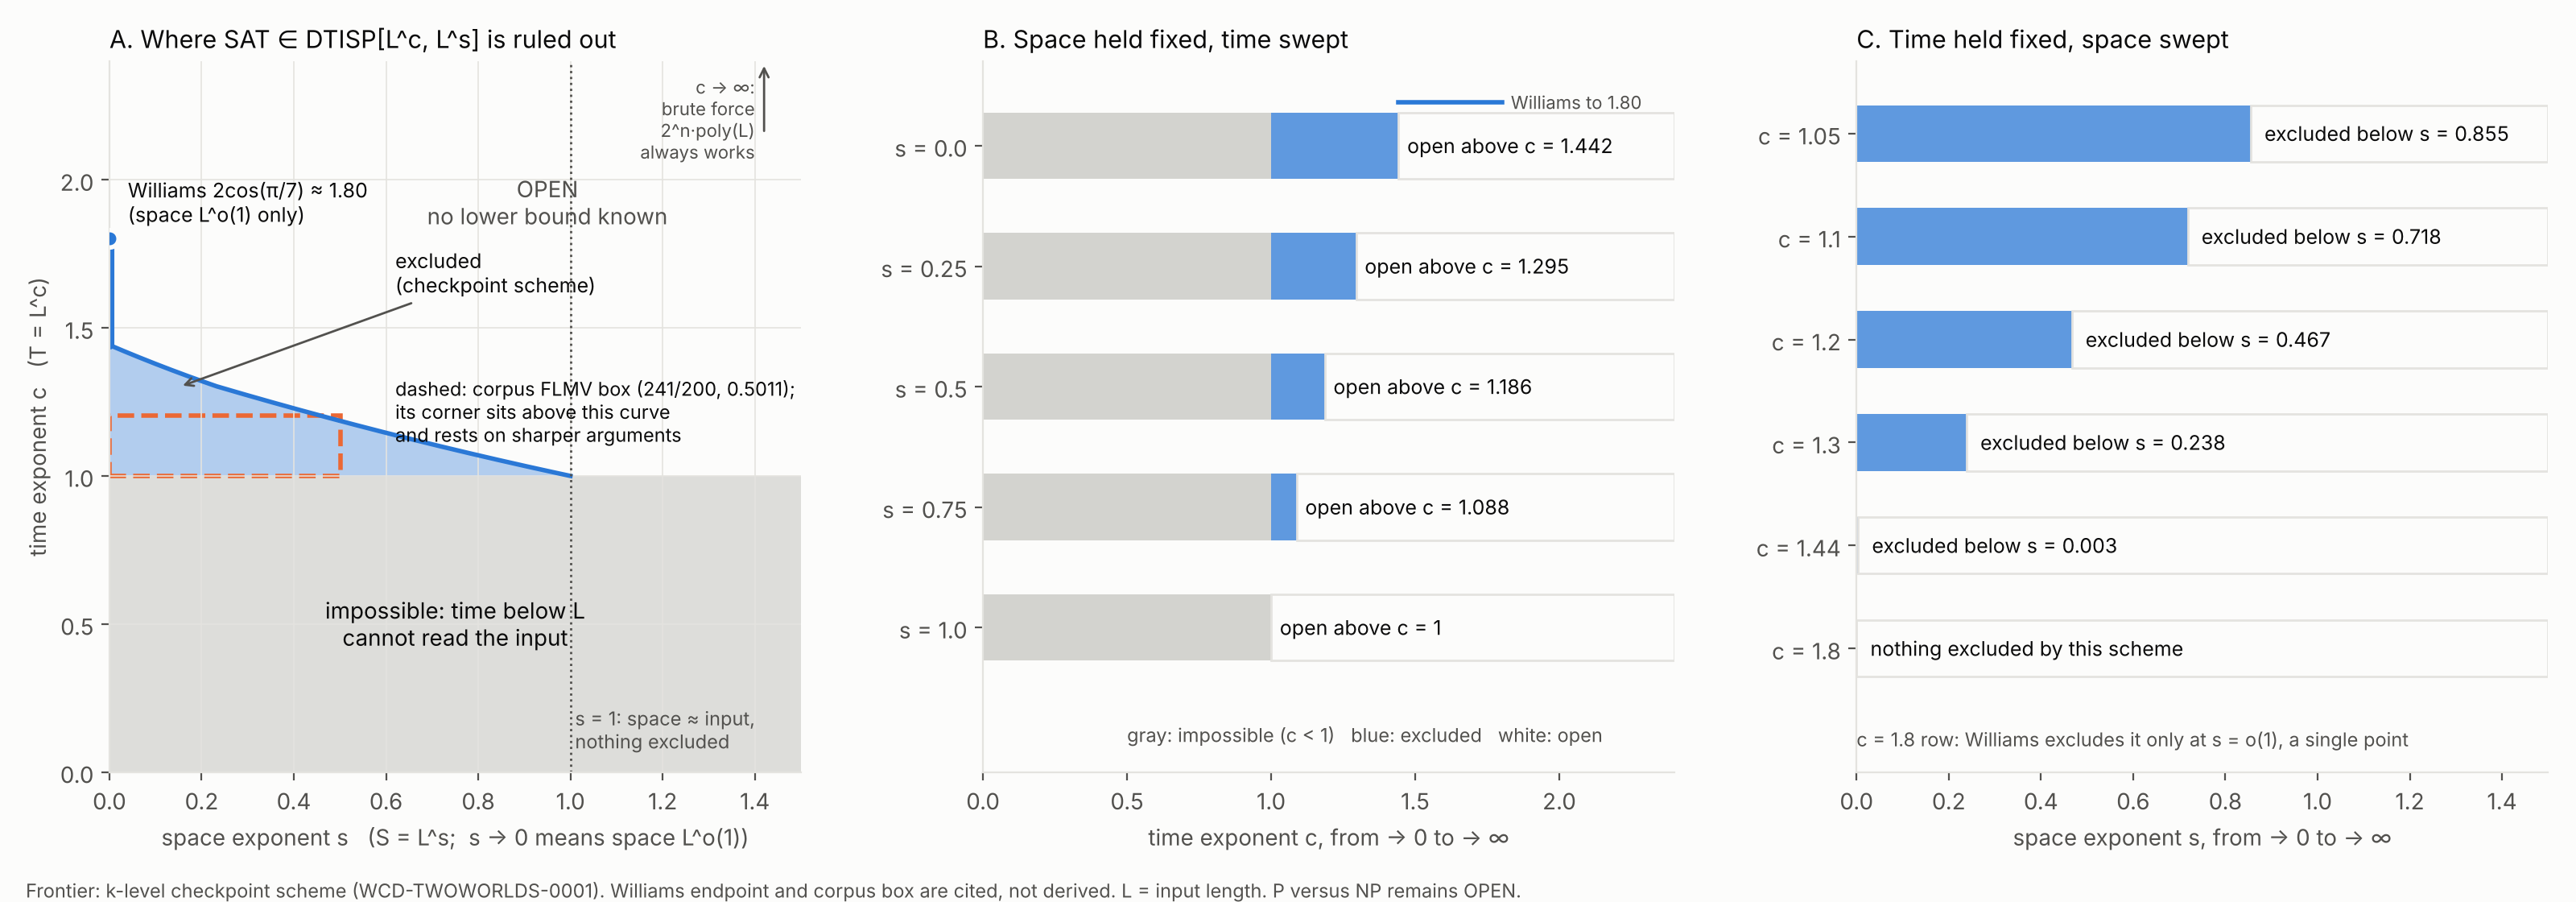
\includegraphics[width=\textwidth]{regimes/flmv_slices.png}
\end{center}
\begin{itemize}
\item \textbf{Panel A.} The plane of exponents $(s,c)$ with $S=L^{s}$, $T=L^{c}$. Below $c=1$ is impossible (Lemma~\ref{lem:skip}). The blue region is excluded by the checkpoint scheme: $c^{k-1}(c+(k-1)s)<k$ for some $k$. The dashed rectangle is the corpus box; its corner lies just above the scheme curve (at $s=0.5$ the curve gives 1.186, the box claims 1.205) and rests on sharper arguments. Williams' endpoint 1.80 holds only at $s=o(1)$.
\item \textbf{Panel B (space fixed, time swept from $\to0$ to $\to\infty$).} At $s=0,0.25,0.5,0.75,1$ the scheme excludes time exponents below $1.442, 1.295, 1.186, 1.088, 1$. Above that nothing is known until brute force, which is exponential.
\item \textbf{Panel C (time fixed, space swept from $\to0$ to $\to\infty$).} At $c=1.05,1.1,1.2,1.3,1.44,1.8$ the scheme excludes space exponents below $0.855, 0.718, 0.467, 0.238, 0.003, 0$. More space never helps a lower bound: every slice becomes open before $s=1$.
\end{itemize}

\section{CORPUS REVIEWED / DUPLICATION AUDIT / CHANGES}
\begin{itemize}
\item \textbf{Corpus reviewed:} the earlier reports of this session; the consolidated living log; the world-ledger pointer in AGENTS.md (rows L13, L38--L40); the ARC/FLMV governance note for the box.
\item \textbf{Duplication / contradiction audit:} no earlier entry of this routine tabulates the parameter limits. The figure frontier reproduces WCD-TWOWORLDS-0001. No contradiction found.
\item \textbf{What changed relative to root main:} nothing; \texttt{main.tex} is not edited.
\item \textbf{Adopted:} the checkpoint frontier; the corpus box as stated by governance. \textbf{Rejected / retired:} none.
\item \textbf{Stale or overstated claims found:} in the chat summary before this report, the dense-regime threshold was given as ``about $0.8\log_2L$ variables''. Lemma~\ref{lem:dense} states it with an unpinned model-dependent constant instead.
\end{itemize}

\section{Evidence}
\texttt{regimes/flmv\_slices\_plot.py} (figure; frontier by bisection over $k=2,\dots,39$), \texttt{regimes/flmv\_slices.png}. Runs in about 2\,s. No TeX engine was available, so this file was not compiled.

\medskip\noindent P versus NP remains OPEN. One OPEN load-bearing arrow means P $\ne$ NP is not proved.
\end{document}
% END_OF_VERIFIED_REPORT::CLAUDE::WCD-REGIMES-0001
